% !TEX root = thesis.tex
\startchapter{Socio-Technical Congruence and Failure}
\label{chap:stc-net2}
Knowing that social networks have an effect on build success opens the next question as to how or more precisely which parts of the social network should be changed to increase the likelihood for a build to succeed.
For this reason we turn to the concept of socio-technical congruence as it postulates that developer should communicate once their work intersects.
Thus in this section we explore the effect of socio-technical networks on build success:

\begin{description}
  \item[RQ 1.2:] Does Socio-Technical Networks influence build success?
\end{description}

Although socio-technical congruence has only been studies in connection with productivity intuitively there should be a connection to software quality such as build success.
For example, imagine two developer modifying classes that share call and data dependencies and one developer making changes that violate certain assumptions the other developer relies on when using the modified code.
This might introduce an error that could have been prevented if both developer would have discussed their work.
Thus, we hypothesize that the concept of socio-technical congruence relates to software quality as well as productivity and might be used to point towards improvements in the social network by pointing out developers that should communicate.

In the remainder of this chapter, we start with detailing the back ground relevant to studying coordination, its influence, and how coordination needs are identified by other researchers (Section~\ref{sec:background}).
Next, we discuss how we calculate socio-technical congruence as well as highlight some modifications to explore to allow us to explore whether a difference in the magnitude of technical dependencies and amount of communication plays a role to possibly highlight improvements for social interactions among software developers (Section~\ref{sec:congruence}).
Subsequently, we briefly go over the methodology that is relevant to exploring our research question that were not mentioned in Chapter~\ref{chap:meth} (Section~\ref{sec:methodology}).
Then, we go over the analysis and results we obtained in Section~\ref{sec:results} followed by a discussion of the results and their implications in Section~\ref{sec:discussion}.
We conclude this chapter with offering an answer to our research question and leading into the subsequent Chapter~\ref{chap:approach} (Section~\ref{sec:conclusion}).


\section{Calculating Congruence}
\label{sec:congruence}
In this section new describe how we derive the socio-technical index as used by Cataldo et al~\cite{cataldo:cscw:2006} from our technical networks by additionally giving some comparison of our approach to the original.

\subsection{Technical Entities and Social Relationships}
A technical entity is an entity in a project that can be worked on by a person. Examples of a technical entity include a source code file, a compiled binary, a requirement, a task, or a bug. Socio-technical congruence has focused on the source code file as the technical entity \cite{cataldo:cscw:2006, ehrlich:stc:2008}, although work has also examined socio-technical congruence using a requirement~\cite{damian2010:rdc,marczak2009:crossfunctional} or a task~\cite{wolf:ieee:2009} as the technical entity. The choice of technical entity depends on the context of the study.

At the core of socio-technical congruence is the concept of a technical dependency. A technical dependency is a type of dependency between two technical entities. Examples of technical dependencies are in Box \ref{ph:technicalunits}.

\begin{placeholder}[t]
\begin{itemize}
\item Requirements that depend on each other~\cite{marczak:re:2008,marczak2009:crossfunctional}
\item Source code modules changed together in a change set~\cite{cataldo:cscw:2006,cataldo:esem:2008}
\item Source code that has a call-graph dependency~\cite{deSouza2004:thwarts_collaboration}
\item Tasks that depend on other tasks \cite{wolf:ieee:2009}
\end{itemize}
\caption{Examples of technical dependencies}
\label{ph:technicalunits}
\end{placeholder}

A coordination need is a relationship that indicates that two people should be coordinating, based on the assignment of each person to a technical entity, and the technical dependencies between the entities.

Social relationships are identified through actual coordination, which indicates how people in the organization are actually coordinating. Note that, despite the nomenclature ``coordination'' used in previous work \cite{cataldo:cscw:2006}, the actual coordination matrix does not need to represent coordination at all, but merely a relationship of interest between two people in an organization. Generally, one would want to choose relationships that are of interest to the performance of the organization, hence favouring the selection of relationships such as ``communication''. Examples of actual coordination appear in Box \ref{ph:relationships}.

\subsection{Calculating Socio-Technical Congruence}
\label{sec:stc}
In Chapter~\ref{chap:meth} we described socio-technical networks and how we conceptualize them in this thesis.
If we reformulate this network into the terms originally used by Cataldo et al~\cite{cataldo:cscw:2006} the matrix representation of the technical dependencies among software developers turns into the coordination needs matrix $CN$ and the social network in matrix representation is the actual coordination matrix $AC$.
Thus we calcite the socio-technical congruence index as follows:

\[ \text{congruence} = \frac{\text{Diff}(CN, AC)}  {|CN|} \]

The main difference to the original formula lies solely in our more direct approach of deriving the coordination needs matrix instead of deriving them from task relationships, that are themselves derived from source code dependencies as we used to directly relate software developers with each othery.

\begin{placeholder}[t]
\begin{itemize}
\item Communication---A communicates with B~\cite{cataldo:cscw:2006, ehrlich:stc:2008, cataldo:esem:2008,damian2007:collaboration}.
\item Location---A is in the same location as B~\cite{cataldo:cscw:2006, ehrlich:stc:2008}.
\item Team structure---A is in the same team as B~\cite{cataldo:cscw:2006}.
\end{itemize}
\caption{Examples of actual coordination}
\label{ph:relationships}
\end{placeholder}


\section{Analysis Methods}
\label{sec:methodology}
Logistic regression is ideal to test the relationship between multiple variables and a binary outcome, which in our study is a build result being either ``OK'' or ``Error''. The presence of many data entities in this project means that we must consider confounding variables in addition to the socio-technical congruence when determining its effects on the probability of build success. Informally, logistic regression identifies the amount of ``influence'' that a variable has in the probability that a build will be successful.
The two main variables we are interested in are as aforementioned the socio-techincal congruence index as well as the ratio between gaps and coordination needs, that is technical dependencies among developers that are not accompanies by a corresponding social dependency.

We show the relationship between a variable and the build success probability by plotting the y-axis as the probability. We use probability because we feel that it is more intuitive than odds ratios or logistic functions. If there is a relationship between a variable and the probability of build success, then we should see that as the variable's value increases, the probability also increases. In the probability figures, the solid line is the expected value, and the dashed lines indicate the 95\% confidence intervals.

We run two different logistic regression models: one using weighted congruence, and one using unweighted congruence. We include the following variables: number of files per build, number of authors contributing to the build, number of files in the build, number of work items per build, the congruence, the build type, and the date of the build. We centre and scale each numeric variable.
Because we were concerned about possible interactions affecting our results, we included first-order interaction effects and used backward stepwise elimination to remove variables to keep AIC (Akaike's Information Criterion) low.

\section{Results}
\label{sec:results}
In the RTC repository, we analyzed 191 builds; of these builds, 60 were error builds, and 131 were OK builds. Table \ref{tab:summary} displays summary statistics per build.
Figure \ref{fig:hist_unweighted_congruence} displays histograms for unweighted congruence, and Figure \ref{fig:hist_unweighted_congruence} shows histograms for weighted congruence. The histograms compare the frequencies for each type of congruence for all builds, the OK builds, and the error builds only. There are some minor differences between unweighted and weighted congruence values; weighted congruence, for instance, largely reduces the number of ``fully'' congruent situations where congruence is 1.

The congruence values are low on average. The unweighted congruence has a mean value of 0.331, and the weighted measure has a mean value of 0.196, meaning that about one-third and one-fifth of the coordination needs are satisfied by actual coordination, respectively. Over 75\% of the builds have a weighted congruence value of less than 0.25.

\begin{figure}[t]
  \centering
  \subfloat[All builds]{
    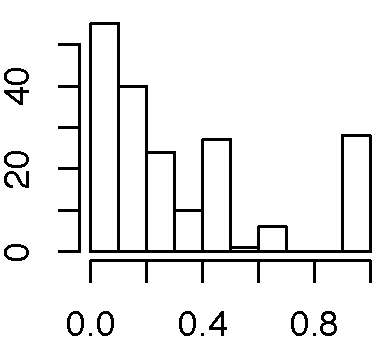
\includegraphics[width=.3\columnwidth]{figures/hist_unweighted}
    \label{subfig:hist_nonweighted}
  }
    \subfloat[OK builds]{
    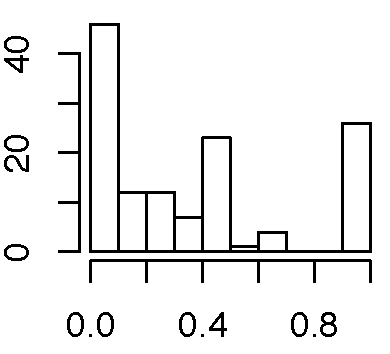
\includegraphics[width=.3\columnwidth]{figures/hist_unweighted_ok}
    \label{subfig:hist_nonweighted_ok}
  }
  \subfloat[Error builds]{
	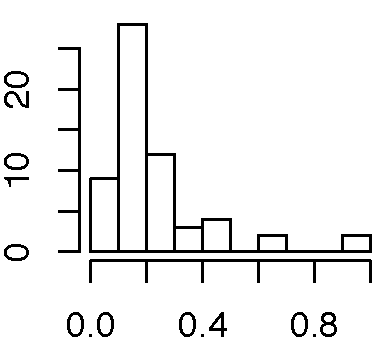
\includegraphics[width=.3\columnwidth]{figures/hist_unweighted_err}
     \label{subfig:hist_weighted_err}
  }
	\caption{Distribution of Congruence Values}
	\label{fig:hist_unweighted_congruence}
\end{figure}

\begin{table}[t]
\centering
\begin{tabular}{lrrrr}
\toprule
 & Min & Median & Max & Mean\\\midrule
Authors & 2 & 17 & 44 & 18.62\\
Files & 5 & 131 & 3101 & 342.3 \\
Change Sets & 4  & 34  & 226 & 54.2\\
Work items & 4 & 34  & 182 & 48.3 \\
Build date range (days) & 0  & 345  & 361 & 319.2 \\
Congruence & 0  & 0.21  & 1 & 0.331 \\
%Gap size & -0.083 & 0.190 & 1.00 & 0.317 \\
\bottomrule
\end{tabular}
\caption{Summary statistics}
\label{tab:summary}
\end{table}

\begin{table}[t]
\begin{center}
\begin{tabular}{lrrrrr}
\toprule
 & 2. & 3. & 4. & 5. & 6. \\ 
  \midrule
   1. Congruence  & -0.27 & -0.22 & -0.33 & 0.08 & 0.19 \\ 
   2. Authors & --& 0.41 & 0.76 & 0.10 & -0.30 \\ 
   3. Files &  & --& 0.37 & 0.08 & -0.20 \\ 
   4. Change sets &  &  &  --& 0.02 & -0.38 \\ 
   5. Work items  &  &  &  &  --& 0.04 \\ 
   6. Build date &  &  &  &  & -- \\ 
\bottomrule

\end{tabular}
\end{center}
\caption{Pairwise Correlation of Variables per Build}
\label{tab:pairwise}
\end{table}

We calculated pairwise correlations between the variables weighted congruence, unweighted congruence, number of authors, number of files, number of change sets, number of work items, and build date (Table \ref{tab:pairwise}). To avoid multicollinearity problems in our data, we choose to remove change sets from our logistic regression analysis because, due to the enforced processes in RTC, we know that there is exactly one author per change set, and thus there is at least as many change sets as authors per build.

To assess the fit of the logistic regression models, we use the Nagelkerke pseudo-$R^2$ and AIC. $R^2$ shows the proportion of variability explained by the model, and AIC is a measure of how well the model fits the data. Ideally, $R^2$ is high and AIC is low. Our current model contains 19 variables and has an $R^2$ of 0.581. We present our model in Table \ref{tab:models} to a model containing every first-order interaction effect with 27 variables and a model that contains the 7 main effects only (in Table \ref{tab:logr_maineffects}). We found that 19 variables is optimal and that removing further variables lowered the $R^2$ value while raising the AIC.

\begin{table}[t]
\begin{center}
\begin{tabular}{l@{\hspace{30pt}}r@{\hspace{30pt}}rr}
\toprule
Model                  & Variables    & AIC & $R^2$                                  \\ \midrule
Every interaction  & 27  & 188.6 & 0.595  \\
Main effects only & 7   & 213.2 & 0.269 \\
\textbf{Our model}         & \textbf{19}  & \textbf{175.8} & \textbf{0.581} \\
\bottomrule
\end{tabular}
\end{center}
\caption{Model comparison}
\label{tab:models}
\end{table}

\subsection{Effects of Congruence on Build Result}
\label{sec:congruence_effect_build_result}

\begin{table}[t]
\begin{center}
\small
\begin{tabular}{l@{\hspace{15pt}}rrr}
\toprule
Variable & Coef. & S.E. & \emph{p} \\
	\midrule
Intercept                   &  -0.5459 &   0.4663 & 0.2417 \\
\textbf{Congruence}              &   \textbf{6.3410} &   \textbf{1.6262} & \textbf{**0.0001} \\
\textbf{Authors}                     &  \textbf{-1.9759} &   \textbf{0.5310} & \textbf{**0.0002}  \\
\textbf{Files}                       &  \textbf{-1.0734} &   \textbf{0.4561} & \textbf{*0.0186}  \\
Work~items                   &  -0.1456 &   0.2355 & 0.5363  \\
\textbf{Build type=I}                      &   \textbf{2.1533} &   \textbf{1.0526} & \textbf{*0.0408}  \\
Build type=N                      &   4.6833 & 200.7587 & 0.9814  \\
Build date                   &  -0.6560 &   0.6709 & 0.3282  \\
\textbf{Congruence * Build type=I}     &  \textbf{-9.2151} &   \textbf{2.5572} & \textbf{**0.0003}  \\
Congruence * Build type=N     &  -7.7308 &  91.8053 & 0.9329  \\
\textbf{Congruence * Build date}  &  \textbf{-5.1266} &   \textbf{1.9290} & \textbf{**0.0079}  \\
Authors $\cdot$ Build type=I            &   1.2688 &   0.7028 & 0.0710  \\
Authors * Build type=N            & 105.4123 & 535.8792 & 0.8441  \\
Authors * Build date         &  -0.6061 &   0.3616 & 0.0937 \\
Authors * Files             &   0.7663 &   0.4289 & 0.0740  \\
Files * Build type=I              &   1.0920 &   1.1838 & 0.3563  \\
Files * Build type=N              & -37.9274 & 199.2314 & 0.8490  \\
\textbf{Work~items * Build date}       &   \textbf{0.8040} &   \textbf{0.3003} & \textbf{**0.0074}  \\
\textbf{Build type=I * Build date}          &   \textbf{2.6442} &   \textbf{0.7678} & \textbf{*0.0006} \\
Build type=N * Build date          &  84.7252 & 344.8129 & 0.8059  \\
	\bottomrule
Model likelihood ratio & 101.92 &  & $R^2=0.581$  \\
& \multicolumn{3}{c}{191 observations}  \\
\multicolumn{1}{l}{ } & \multicolumn{3}{l}{\scriptsize{Build type is set to continuous}} \\
\multicolumn{1}{l}{\scriptsize{*$p < 0.05$; **$p < 0.01$}} & \multicolumn{3}{l}{\scriptsize{Nagelkerke is used as the pseudo-$R^2$ measure}}
\end{tabular}
\end{center}
\caption{Logistic Regression models predicting build success probability with main and interaction effects}
\label{tab:logr}
\end{table}


\begin{table}[t]
\begin{center}
\begin{tabular}{l@{\hspace{15pt}}rr r}
\toprule
Variable & Coef. & S.E. & \emph{p} \\
	\midrule                                                                
	Intercept                &  0.5265 & 0.3040 & 0.0833 \\
	Congruence               &  0.9371 & 0.6807 & 0.1686 \\
	\textbf{Authors}         & \textbf{-0.5702} & \textbf{0.2003} & \textbf{**0.0044}  \\
	\textbf{Files}           & \textbf{-0.6398} & \textbf{0.2477} & \textbf{**0.0098} \\
	Work~items                & -0.1755 & 0.1713 & 0.3055  \\
	Build type=I                   &  0.1693 & 0.4269 & 0.6917  \\
	Build type=N                   &  0.2133 & 0.7791 & 0.7842  \\
	Build date               & -0.1331 & 0.1821 & 0.4649  \\
	\bottomrule
Model likelihood ratio & 40.59 &  & $R^2=0.269$  \\
& \multicolumn{3}{c}{191 observations}  \\
\multicolumn{1}{l}{ } & \multicolumn{3}{l}{\scriptsize{Build type is set to continuous}} \\
\multicolumn{1}{l}{\scriptsize{*$p < 0.05$; **$p < 0.01$}} & \multicolumn{3}{l}{\scriptsize{Nagelkerke is used as the pseudo-$R^2$ measure}}
\end{tabular}
\end{center}
\caption{Logistic Regression models predicting build success probability with main effects only}
\label{tab:logr_maineffects}
\end{table}

The result of logistic regression indicates that the following effects are significant for both unweighted and weighted congruence models: The congruence~$\times$~build type effect, the congruence~$\times$~build date interaction effect, the number of work~items~$\times$~build date interaction effect, and the build date~$\times$~build type effect. In addition, the number of authors and the number of files are significant main effects, although their coefficients are lower than the interaction effects involving congruence. We also identify unweighted congruence as a significant main effects in the unweighted congruence model (see Table~\ref{tab:logr}).

In the next section we discuss the main effects and interactions effects that involve congruence affecting build probability. We discuss the effects of the non-congruence effects, including the authors, files, work~items~$\times$~date interaction effect and the date~$\times$~nightly~build effect in Section \ref{sec:otherfactors}.

\subsubsection{Effects of interactions involving congruence}
\label{sec:congruenceinteractions}
The type~$\times$~congruence interaction effect, the date~$\times$~congruence interaction, and the type $\times$ date effect are each significant in our model (Table \ref{tab:logr}). We plot in Figure~\ref{fig:unweighted_congruence_typeci_age} the effects of congruence vs. probability of build success at the 10\% date quantile (2008-01-25), at the 25\% date quantile (2008-05-14), the 50\% date quantile (2008-06-07), and the latest build (2008-06-26).


\begin{figure}[t!]
\centering
  \subfloat[ \small{2008-01-25} ]{
    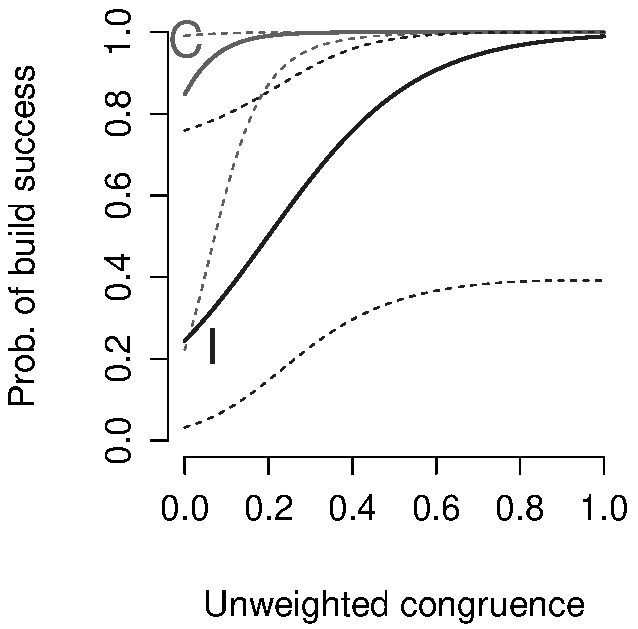
\includegraphics[width=.4\columnwidth]{figures/prob_unweighted_age_typeci_q010}
    \label{subfig:prob_unweighted_age_typeci_q010}
  }
  \subfloat[ \small{2008-05-14} ]{
	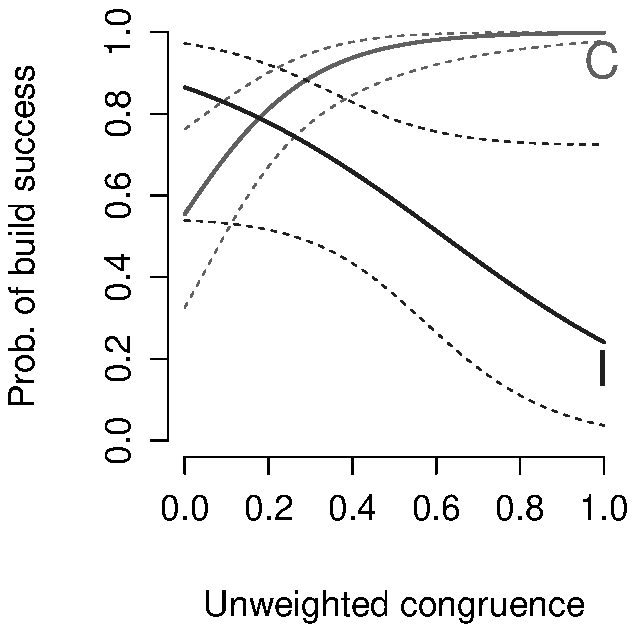
\includegraphics[width=.4\columnwidth]{figures/prob_unweighted_age_typeci_q025}
     \label{subfig:prob_unweighted_age_typeci_q025}
  }
  
  \subfloat[ \small{2008-06-07} ]{
	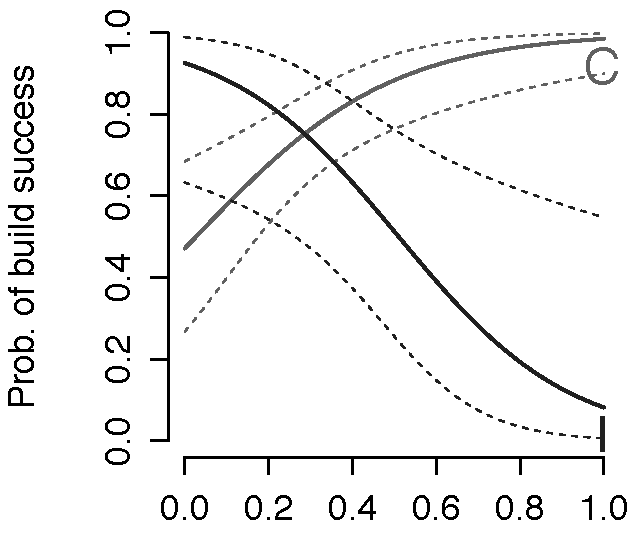
\includegraphics[width=.4\columnwidth]{figures/prob_unweighted_age_typeci_q050}
     \label{subfig:prob_unweighted_age_typeci_q050}
  }
  \subfloat[ \small{2008-06-26} ]{
	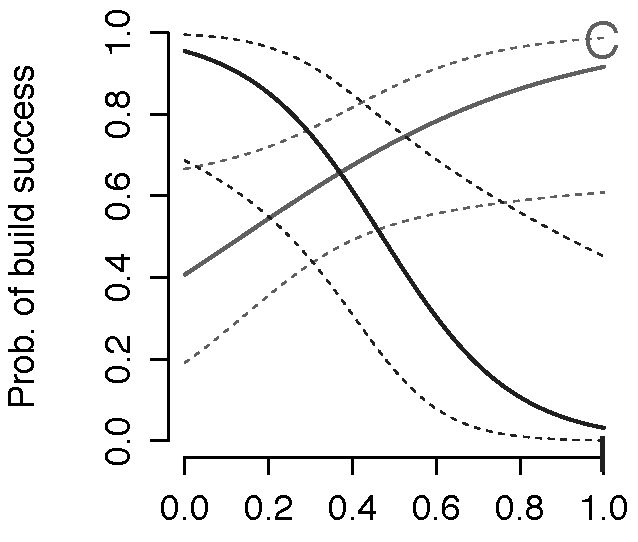
\includegraphics[width=.4\columnwidth]{figures/prob_unweighted_age_typeci_q100}
     \label{subfig:prob_unweighted_age_typeci_q100}
  }
  
	\caption{Estimated probability of build success for \emph{congruence} and \emph{continuous builds C} or \emph{integration builds I}  over time, adjusted to authors $\approx$ -0.156 (17 authors), files $\approx$ -0.352 (131 files), work~items $\approx$ -0.399 (34 work items)}
	\label{fig:unweighted_congruence_typeci_age}
\end{figure}

The congruence model (Table \ref{tab:logr}) the effect of congruence on continuous builds is significant, and that increasing congruence also increases the probability that a continuous build will succeed. 
For integration builds (Figures \ref{fig:unweighted_congruence_typeci_age}, in black), an increase in congruence decreases build success, with the exception of the 2008-01-25 build (Figure \ref{subfig:prob_unweighted_age_typeci_q010}). In in our 2008-01-25 build, we see that low congruence leads to low build probability, but high congruence has high build probability. As the project ages, this trend reverses and congruence is clearly inversely related with build success probability (Figure \ref{subfig:prob_unweighted_age_typeci_q100}).
The effect of congruence is totally opposite for continuous builds and integration builds. Based on Figure \ref{subfig:prob_unweighted_age_typeci_q100}, increasing congruence significantly improves the continuous build success rate. However, increasing congruence significantly decreases the integration build success rate.


\subsection{Effect of Gap Ratio on Build Result}
\label{sec:gapsizeresult}
We build logistic regression models based on the model in Table \ref{tab:logr} using the gap ratio measurement (percentage of unmet coordination needs) . In the interest of saving space, we report only the odds ratio. We retain every significant interaction from our previous weighted congruence logistic regression in Table \ref{tab:logr}.

The effect of gap ratio on build result is significant (Table \ref{tab:oddsratio_gapsize}). This indicates that increasing the gaps ratio significantly increases the odds that an OK build will occur, which is the opposite of what we hypothesized (Figure \ref{fig:prob_gapsize_a}). This means that if the gap size is large, the build success probability increases.

\begin{table}[t]
\begin{center}
\begin{tabular}{lrr}
  \toprule
 & Model\\ 
  \midrule
Intercept & 1.32 \\ 
  Authors &  0.60 \\ 
  Files &  0.63 \\ 
  Work~items  & 0.85 \\ 
  Build type=I  & 1.31 \\ 
%  Weighted cong & 8.41 & - \\ 
  Gap ratio  & 8.71 \\ 
  Build date  & 0.59 \\ 
  Authors * Build date & 0.74 \\ 
  Work~items * Build date  & 1.83 \\ 
  Build type=I * Build date  & 2.52 \\ 
%  Build type=I * Weighted cong & 0.01 & - \\ 
%  Weighted cong * Build date & 0.00 & - \\ 
   \bottomrule
\end{tabular}
\caption{Odds Ratio for Gap Ratio Models}
\label{tab:oddsratio_gapsize}
\end{center}
\end{table}


\begin{figure}[t]
	\centering	
	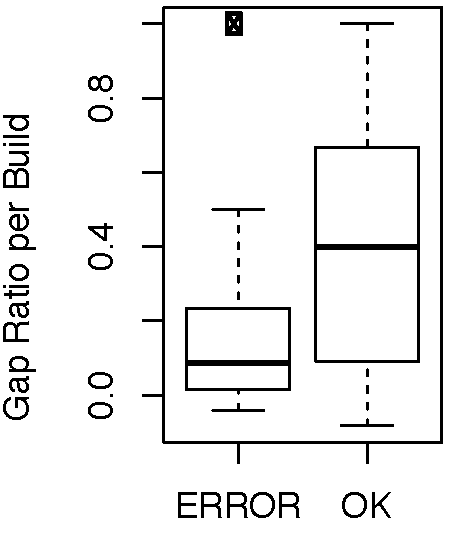
\includegraphics[width=.5\columnwidth]{figures/boxplot_meangapsize}
	\caption{Gap Ratio per Build}
	\label{fig:gapsizes}
\end{figure}

\begin{figure}[t]
	\centering
	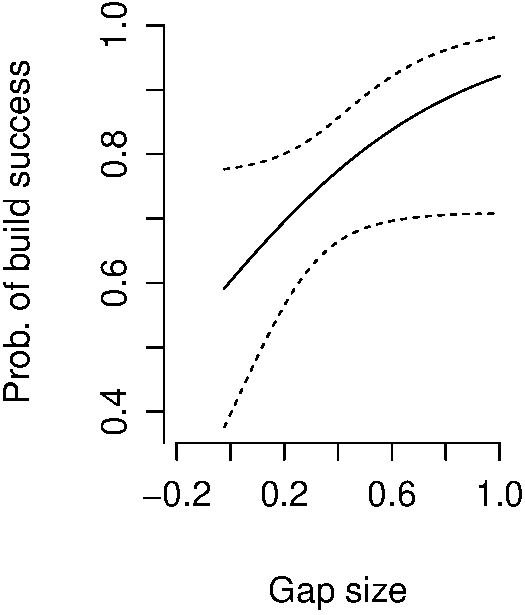
\includegraphics[width=.5\columnwidth]{figures/prob_gapsize_g1}
	\caption{Effect of gap ratio on build success probability. }
	\label{fig:prob_gapsize_a}
\end{figure}




\subsection{Social and Technical Factors in RTC Affecting Build Success and Congruence}
\label{sec:otherfactors}
In light of our results, we examine not only the number of work~items~$\times$~date significant interaction found in Section \ref{sec:congruence_effect_build_result}, but different social and technical factors that may affect congruence
and build success probability to find explanations for the interactions between socio-technical congruence and build success probability in RTC.
Specifically, we examine the effect of build date on work items, coordination around fully-congruent builds and
incongruent builds, and the effects of commenting behaviour on builds.

\subsubsection{Other Effects on Build Success}
\label{sec:effectauthors}
\begin{description}
\item[Authors] As the number of authors involved in a build increases, the probability that the build succeeds decreases. The build probability is significantly lowered after more than 15 authors are involved in the build (Figure \ref{subfig:prob_weighted_authors_age_q100}). When over 30 authors are involved in the build, the estimated build success probability falls under 10\%.

\item[Files] As the number of files involved in a build increases, the probability that the build will succeed decreases (Figure \ref{subfig:prob_weighted_files_age_q100}).

\item[Build Date and Work items] The work~items~$\times$~date interaction is significant. Early in the project, as the number of work items increases, the probability of build success decreases (Figure \ref{subfig:prob_weighted_workitems_age_q010}). As the project ages, this trend reverses and as the number of work items increases, the probability of build success increases as well (Figure \ref{subfig:prob_weighted_workitems_age_q100}). According to the coefficients in Table \ref{tab:logr}, this effect on build success probability is not as strong as the authors main effect or the files main effect.
\end{description}

\begin{figure}[t]
\centering
\subfloat[ \small{Authors} ] {
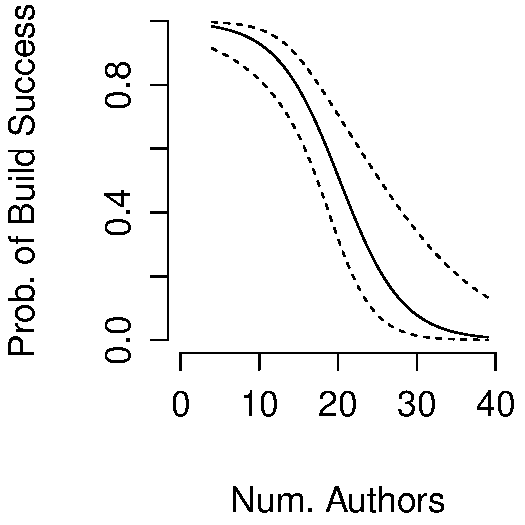
\includegraphics[width=.45\columnwidth]{figures/prob_weighted_authors_age_q100}
\label{subfig:prob_weighted_authors_age_q100}
}
\subfloat[ \small{Files} ] {
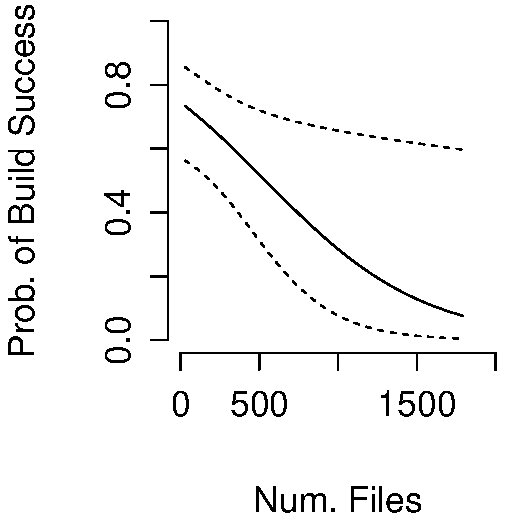
\includegraphics[width=.45\columnwidth]{figures/prob_weighted_files_age_q100}
\label{subfig:prob_weighted_files_age_q100}
}

\caption{Estimated probability of build success for \emph{authors} and \emph{files},  congruence. Adjusted to work~items $\approx$ -0.399 (34), authors $\approx$ -0.156 (17), files $\approx$ -0.352 (131), congruence $\approx$ 0.1446, type = cont, date=2008-06-26}
  \label{fig:weighted_congruence_authors_age}
\end{figure}



\begin{figure}[t]
\centering
  \subfloat[ \small{2008-01-25} ]{
    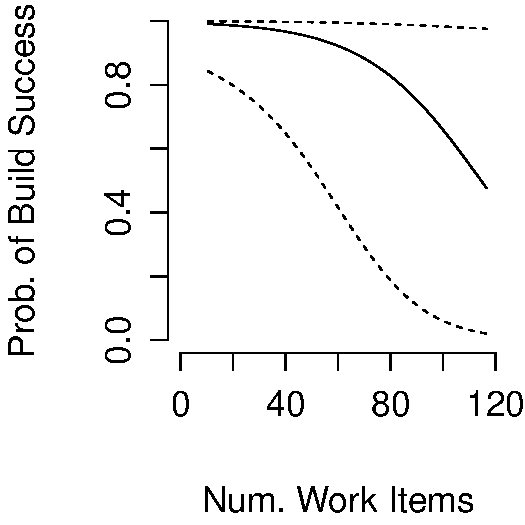
\includegraphics[width=.45\columnwidth]{figures/prob_weighted_workitems_x_age_q010}
    \label{subfig:prob_weighted_workitems_age_q010}
  }
  \subfloat[ \small{2008-06-26} ]{
	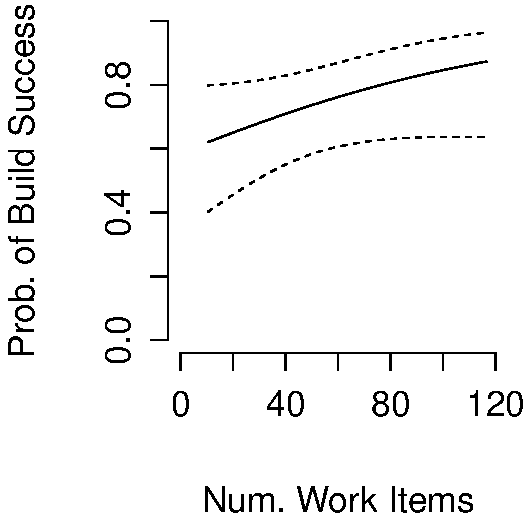
\includegraphics[width=.45\columnwidth]{figures/prob_weighted_workitems_x_age_q100}
     \label{subfig:prob_weighted_workitems_age_q100}
  }
  \caption{Estimated probability of build success for \emph{work items} and \emph{date},  congruence. Adjusted to authors $\approx$ -0.156 (17), files $\approx$ -0.352 (131), congruence $\approx$ 0.1446, type = cont}
  \label{fig:weighted_congruence_workitems_age}
\end{figure}

\subsubsection{Examining Extreme Congruence Values}
\label{sec:extremecongruence}
We are interested in the differences between high-congruence builds and low-congruence builds.
We further this investigation by looking at builds that have extreme values of congruence: zero, where absolutely no coordination needs are satisfied with communication, and one, where every coordination need is satisfied with communication.
We chose to investigate the extreme cases to see if there were differences in the way people coordinated in fully-congruent builds, and in incongruent builds.
Table \ref{tab:congruence_extremes} shows the number of OK and error builds that occurred when congruence was equal to one, and equal to zero. The weighted builds with full congruence are a subset of the unweighted builds with full congruence.


\begin{table}[t]
\centering
\begin{tabular}{llrr}
\toprule
& & \multicolumn{2}{c}{Congruence} \\\midrule
&  & 1 & 0 \\\midrule
\multirow{2}{*}{Unweighted} & OK & 26 & 30 \\
                            & ERR & 2 & 2 \\%\midrule
%\multirow{2}{*}{Weighted} & OK & 6 & 30 \\
 %                        & ERR & 1 & 2 \\
 \bottomrule
\end{tabular}
\caption{Number of Builds with Congruence Values 0 and 1}
\label{tab:congruence_extremes}
\end{table}

To determine if the presence of commenting affected the builds, we examined the number of comments on work item--change set pairs in builds with extreme unweighted congruence values. Our results are shown in Table \ref{tab:changeset_commenters}. Build success probabilities improve with respect to builds that have no comments, though work items with no comments are in the minority.

Of note is the high number of comments on work items that have zero congruence. This indicates that individuals who have no technical relationship to the work item are commenting on the work item.

\begin{table}[t]
\centering
\begin{tabular}{ll@{\hspace{40pt}}rr@{\hspace{40pt}}rr}
\toprule
& & \multicolumn{2}{@{\hspace{-40pt}}c}{Num. of Pairs} & \multicolumn{2}{c}{Success rate} \\
Congruence &                                & 1     & 0   & 1 & 0 \\\midrule 
\multirow{2}{*}{No comments} 	& OK 	  & 42   & 143  &  \multirow{2}{*}{49\%} & \multirow{2}{*}{69\%}  \\
                            	& Error   & 43    & 64   &  & \\\midrule
\multirow{2}{*}{Comments} 	& OK 	  & 610  & 445  & \multirow{2}{*}{68\%} & \multirow{2}{*}{69\%}  \\
                         	& Error   & 290   & 199  &  & \\\midrule
\multirow{2}{*}{Total} 		& OK		  & 652 & 588 &     \multirow{2}{*}{66\%} & \multirow{2}{*}{69\%}   \\
                       		& Error   & 333  & 263 & &\\\bottomrule
\end{tabular}
\caption{Number of work items-change set pairs with comments and build success probabilities for congruence 0 and 1}
\label{tab:changeset_commenters}
\end{table}

We manually inspected the work items with extreme amounts of congruence, reading the comments for any differences in the content discussed. Unfortunately, there were no obvious qualities between comments made in a build with a congruence of zero, and comments made in a build with a congruence of one. In both builds, individuals discussed technical implementation details, provided updates to colleagues, or requested assistance from colleagues. We are unable to discover root causes of failure without a deeper examination of the technical changes and more knowledge of the RTC context.


\section{Discussion}
\label{sec:discussion}
The concepts illustrated in Conway's Law, as well as previous empirical work on socio-technical congruence lead us to expect that team members must coordinate according to coordination needs suggested by technical dependencies in order to build software effectively.
In this case study, we applied socio-technical congruence to study coordination and its relationship to build success probability in RTC. We applied a modified weighted congruence measurement to study also how the size of a coordination gap affects build success probability, and investigated what social and technical factors in RTC affect congruence and builds.

Overall, we found that the average congruence across builds was very low---only 20--30\% of the coordination needs in the project were fulfilled with actual coordination. Even in the cases where there is zero congruence, the build result was an OK build in over 90\% of the observed cases.

We found that there was an interaction effect involving congruence and build type on build success probabilities (Section \ref{sec:congruenceinteractions}). For continuous builds, increasing congruence improves the chance of build success in continuous builds and can actually decrease build success probability in integration builds (Figures \ref{fig:unweighted_congruence_typeci_age}). High unweighted congruence significantly improves continuous build success probability, and both unweighted and weighted congruence significantly reduce integration build success probability.

The gap ratio is a representation of whether enough coordination
occurred to fulfill multiple coordination needs. If two developers have multiple dependencies on each other, one would expect them to
coordinate more often as well.
We hypothesized that a small gap ratio would increase the probability of successful builds and that a large gap ratio would decrease the probability of a successful build. Instead, we found that as the mean gap size increases, the build success probability also increases (Figure \ref{fig:prob_gapsize_a}).

Below we discuss the reasons for these observed results based on our knowledge of RTC.

\subsection{Strong Awareness Helps Coordination}
The overall congruence for the majority of builds is low: over 75\% of
builds have a congruence of less than 0.25 (Section \ref{sec:congruence_effect_build_result}).
Despite low congruence, the RTC team is able to successfully build its software in many situations.

When we examined extreme congruence values, we observed 85\% build success probability when weighted congruence is 1 and 93\% build success when weighted congruence is 0 (Section \ref{sec:extremecongruence}).
If socio-technical congruence is a measure of coordination quality in software, and builds rely on coordination quality to be successful, then there must be reasons why builds can succeed even when the congruence is zero.

First, because RTC is a highly-distributed project, the product under development uses a modular design \cite{maccormack2006} and thus is affected less by dependencies. Second, team members in RTC do not conduct all of their coordination through \emph{explicit communication} even though work item inspection and discussion with developers indicate that the RTC corporate culture focuses on the work item as their base for communication. Rather, they use the \emph{shared workspace} that incorporates cues from the environment and from peers in order to address technical issues. Both of these effects may contribute to congruence being lower than expected.

\subsubsection{RTC supports Explicit Communication}
The RTC team members use the RTC environment extensively to communicate with each other. We were informed that RTC team members rarely use private email, and our inspection of the mailing list reveals that its primary purpose is for announcements such as server outages rather than for discussing technical work.

This leaves the RTC work item comment system and instant messaging as methods for communication, as well as the phone and internal face-to-face meetings.
We learned that while face-to-face interaction is efficient for solving local issues, it does not benefit remote teams, and the RTC team as a whole encourages every team member to record face-to-face discussions as comments for the purpose of archiving and sharing information.

However, explicit coordination has a cost. There is evidence that involving too many authors in the same build also reduces the build success when using a weighted congruence conceptualization (Figure \ref{subfig:prob_weighted_authors_age_q100}); the effect for unweighted congruence is similar. The overhead required to coordinate many people may interfere with the ability of the team to build the project successfully, suggesting that there is a limit before a developer is overloaded with information.

\subsubsection{RTC is a Shared Workspace}
The RTC client software helps a developer acquire and maintain \emph{environmental awareness} of what is going on in the project by providing access to a shared workspace. Much of the work is centred around the RTC technical entities, which include plans, source code, work items, and comments.
RTC's awareness mechanisms feature a developer-centred dashboard that reports changes to the workspace, built-in traceability, user notifications, regularly-generated reports, and an optional web browser interface. For example, when a change set is created, it is attached to a work item, thus ensuring that people who are involved with the work item receive notification of this change set. These automatic notifications cut down the amount of explicit communication and allow people to coordinate implicitly.

Coordinating using the workspace is well-known in the computer-supported cooperative work domain \cite{schmidt1996}. Open-source developers, in particular, coordinate around source code~\cite{bolici:stc:2009} and mailing lists \cite{gutwin2004:awareness,mockus2002:opensource} because there is little opportunity for face-to-face interaction. RTC shares many characteristics with open-source development, such as a distributed team and a transparent development process.

In light of these results, we believe that, using our conceptualization, the RTC team requires a congruence of only 0.2--0.3 for their tasks to be completed.
Much of the need for explicit, point-to-point communication is mitigated by implicit communication and the use of the workspace to coordinate.
We expect that the remaining congruence is covered through the RTC workspace, and through face-to-face communication, instant messenger, and phone communication. Though our congruence value appears low for the RTC team, the coordination in reality may be higher. Future studies should keep in mind that congruence may be lower than expected because of conceptualizations that cannot include every type of coordination in a project.

\subsection{Coordination and Geographic Distribution}
As RTC is a distributed team, geographic distribution has an effect on team performance, though the RTC environment helps mitigate some of these effects \cite{Nguyen:2008Distance}.

We learned from the RTC project that continuous and nightly builds should involve mainly a co-located team, and that integration builds involve multiple components from RTC teams in different locations. Our results suggest that congruence best benefits builds that occur within co-located teams; however, the design of our study does not allow us to draw a firm conclusion about the influence of both co-location and congruence on build success probability.

It appears that involving too many individuals when coordinating the activities of various teams may harm build success due to information overload~\cite{damian:icgse:2007}, especially when the team members are distributed. To negate this effect, development leaders and build managers that have an overall view of the project are suited to coordinate teams to ensure build success \cite{hinds:cscw:2006}.


\subsection{Project Maturity and Build Success}
We found that early builds exhibited a different type of relationship between congruence and build success probability than later builds (Section \ref{sec:congruenceinteractions}). Over the course of the study, we observed 13 internal milestones; the last milestone in our observed builds was a public beta release for end users.

Build success probability decreased significantly over time for continuous builds and stayed roughly the same for integration builds (Figures \ref{fig:unweighted_congruence_typeci_age}).
However, the early builds in the project behaved contrary to later builds in the project (Figure \ref{subfig:prob_unweighted_age_typeci_q010} and \ref{subfig:prob_unweighted_age_typeci_q010}). The RTC software early in its lifetime is in a state of change. Integration builds are not a priority, and features are being added to the project. This means that dependencies are changing rapidly, as well as the expertise among team members, making it difficult to solidify coordination needs.

In addition to interactions between congruence and type, and congruence and date, we observed a significant interaction effect between build date and work items.
We found that early in the project (Figure \ref{subfig:prob_weighted_workitems_age_q010}), builds with large numbers of work items have a high probability of failing, but late in the project (Figure \ref{subfig:prob_weighted_workitems_age_q100}), these builds succeed. Because the latest release was focused on a public release, a build linked to numerous work items may indicate that a bug is highly problematic or a feature is highly desired, and therefore received more attention. 



\section{Conclusion}
\label{sec:conclusion}
We end this chapter by bringing it back to the initial research question we set out to answer:
\begin{description}
  \item[RQ 1.2:] Does Socio-Technical Networks influence build success?
\end{description}

We conducted two investigations: (1) the investigation the influence of the socio-technical congruence index on build success and (2) the investigation of gaps uncovered by socio-technical networks and their influence on build success.
Both avenues of investigations showed that they expose an influence on build success even in the presence of other measures of build size.

These findings, especially that gaps within socio-technical networks influence build success, opens the door to formulating an approach on how to leverage the concept of socio-technical congruence to improve the communication among software developers.
Thus in the next chapter we will detail an approach that we propose to improve developer communication using the concept of socio-technical congruence.
